\documentclass[11pt]{article}
\usepackage[T1]{fontenc}
\usepackage[utf8]{inputenc}
\usepackage{lmodern}
\usepackage[margin=1in]{geometry}
\usepackage{microtype}
\usepackage{amsmath,amssymb,amsthm,mathtools}
\usepackage{enumitem}
\usepackage{xcolor}
\usepackage{hyperref}
\usepackage{booktabs}
\usepackage{array}
\usepackage{tikz}
\usetikzlibrary{arrows.meta,positioning,calc,fit}
\hypersetup{colorlinks=true,linkcolor=blue!45!black,citecolor=blue!45!black,urlcolor=blue!45!black}

\definecolor{accent}{RGB}{35,73,119}
\definecolor{lightaccent}{RGB}{237,243,250}
\definecolor{rulegray}{RGB}{92,104,116}

\setlength{\parindent}{0pt}
\setlength{\parskip}{0.55em}
\setlist[itemize]{topsep=0.3em,itemsep=0.15em,leftmargin=1.5em}
\setlist[enumerate]{topsep=0.3em,itemsep=0.15em,leftmargin=1.8em}

\newtheorem{theorem}{Theorem}[section]
\newtheorem{lemma}[theorem]{Lemma}
\newtheorem{proposition}[theorem]{Proposition}
\newtheorem{corollary}[theorem]{Corollary}
\theoremstyle{definition}
\newtheorem{definition}[theorem]{Definition}
\newtheorem{remark}[theorem]{Remark}
\newtheorem{example}[theorem]{Example}

\newcommand{\ALCIRCC}{\mathsf{ALCI\_RCC5}}
\newcommand{\cl}{\operatorname{cl}}
\newcommand{\tp}{\operatorname{tp}}
\newcommand{\Ex}{\operatorname{Ex}}
\newcommand{\Roles}{\mathsf{R}}
\newcommand{\Eq}{\mathsf{EQ}}
\newcommand{\Dr}{\mathsf{DR}}
\newcommand{\Po}{\mathsf{PO}}
\newcommand{\Pp}{\mathsf{PP}}
\newcommand{\Ppi}{\mathsf{PPI}}
\newcommand{\inv}{\operatorname{inv}}
\newcommand{\Succ}{\operatorname{Succ}}
\newcommand{\repr}{\operatorname{repr}}
\newcommand{\lca}{\operatorname{lca}}
\newcommand{\occ}{\operatorname{Occ}}
\newcommand{\width}{\operatorname{width}}
\newcommand{\state}[1]{\mathsf{#1}}

\title{\textbf{A Contextual Tableau Calculus for $\ALCIRCC$}\\[0.4em]
\large Local state rules, global caching, and an unfolding soundness theorem}
\author{Prepared by GPT-5.4 Pro}
\date{March 2026}

\begin{document}
\maketitle

\begin{abstract}
This note turns the earlier deterministic-mosaic idea into an explicit tableau-style formalism. A tableau node is not a single individual with a unary label. Instead it is a finite \emph{contextual local state}: a finite atomic RCC5 network of remembered items around a distinguished center, together with one designated witness item for each existential demand of the center. Tableau expansion then has two layers. The local rules saturate a single state by boolean closure, universal propagation, transitive-role propagation, witness creation, and RCC5 path-consistency checks. The global rules attach to every remembered item a successor state centered at that item and equip each such edge with a recentering map back into the parent state. Global caching identifies isomorphic saturated local states.

I prove the main soundness statement in full: every open finite tableau graph unfolds into a genuine strong-$\Eq$ model of the input concept. Completeness is isolated as a finite-width extraction problem: if every satisfiable concept has a finite closed family of bounded-width local states, then the corresponding $N$-tableau is complete. So the present note does not claim a finished decidability proof by itself. It does, however, provide a precise tableau architecture that makes the remaining proof obligation explicit.
\end{abstract}

\section{Introduction}

Wessel's original report introduced the $\mathsf{ALCIRCC}$ family and left the decidability of $\mathsf{ALCIRCC5}$ open while noting that ordinary DL tableau methods do not fit the setting well: models are complete graphs, $\Pp$-chains can force infinite models, and a useful calculus would need a stronger blocking or ``infinity checker'' mechanism \cite{Wessel2003}. A later 2026 discussion draft proposed a complete-graph tableau with blocking on unary labels, but that loses witness identity and does not seem strong enough for the full logic as stated \cite{Claude2026}.

The natural repair is to change the shape of a tableau node. In this note, a tableau node is not an individual. It is a finite local \emph{context state}. The state remembers:
\begin{itemize}
    \item the closure-type of a distinguished center item,
    \item one designated witness item for each existential demand of the center,
    \item the exact RCC5 relations between all remembered items, and
    \item for every remembered item, a successor state centered at that item together with a recentering map back into the current state.
\end{itemize}

This is a tableau reformulation of the deterministic witness-indexed mosaic idea from the previous draft, but now presented as an explicit calculus with local and global rules.

The output of the search is a finite rooted directed graph of saturated local states. I call such an object an \emph{open $N$-tableau graph}, where $N$ bounds the maximum number of remembered items in any state. The key formal results of the note are:
\begin{enumerate}
    \item a precise definition of local tableau states and their rule obligations;
    \item an equivalence between open $N$-tableau graphs and finite closed families of width at most $N$;
    \item an unfolding theorem showing that every open tableau graph yields a genuine strong-$\Eq$ model;
    \item a conditional completeness statement: if every satisfiable concept admits such a finite closed family at some computable width bound $N(C)$, then the tableau is a terminating decision procedure.
\end{enumerate}

So this note should be read as a more formal tableau architecture, not as a claim that the last model-extraction lemma is already settled.

\section{Preliminaries}

\subsection{Roles and strong $\Eq$ semantics}

Throughout, the RCC5 role alphabet is
\[
\Roles = \{\Dr,\Po,\Eq,\Pp,\Ppi\}.
\]
The converse operation satisfies
\[
\inv(\Dr)=\Dr,\qquad \inv(\Po)=\Po,\qquad \inv(\Eq)=\Eq,\qquad \inv(\Pp)=\Ppi,\qquad \inv(\Ppi)=\Pp.
\]

I work under the strong $\Eq$ semantics from Wessel's report \cite{Wessel2003}: in every intended model,
\[
\Eq^{\mathcal I}=\{(x,x):x\in \Delta^{\mathcal I}\}.
\]
All pairs satisfy the one-cluster, JEPD, converse, and RCC5 composition conditions.

\subsection{Eliminating modal uses of $\Eq$}

Because $\Eq$ is identity under the strong semantics,
\[
\exists \Eq.D \equiv D
\qquad\text{and}\qquad
\forall \Eq.D \equiv D.
\]
I therefore preprocess the input concept $C$ by replacing every modal occurrence of $\Eq$ by the corresponding subformula. After this normalization, the only modal roles that still appear in formulas are
\[
\Roles^- = \{\Dr,\Po,\Pp,\Ppi\}.
\]
The frame semantics still uses $\Eq$, but the syntax of the satisfiability problem does not.

\subsection{Closure and Hintikka types}

Fix a normalized input concept $C$ in negation normal form.

\begin{definition}[closure]
$\cl(C)$ is the closure of $C$ under subformulas, together with $\neg A$ whenever the concept name $A$ occurs in $C$.
\end{definition}

\begin{definition}[Hintikka type]
A set $\tau\subseteq \cl(C)$ is a \emph{Hintikka type} if:
\begin{enumerate}[label=(T\arabic*)]
    \item if $D_1\sqcap D_2\in \tau$, then $D_1,D_2\in \tau$;
    \item if $D_1\sqcup D_2\in \tau$, then $D_1\in \tau$ or $D_2\in \tau$;
    \item for every concept name $A$ occurring in $\cl(C)$, exactly one of $A$ and $\neg A$ lies in $\tau$.
\end{enumerate}
\end{definition}

For an element $a$ of a model $\mathcal I$, write
\[
\tp_{\mathcal I}(a)=\{D\in \cl(C): a\in D^{\mathcal I}\}.
\]
Only finitely many Hintikka types exist.

\begin{definition}[transitive universal closure]
For a type $\tau$, let
\[
\mathsf{TrUniv}(\tau)=\{\forall \Pp.D,\forall \Ppi.D\in \tau\}.
\]
These are the universal formulas whose role is transitive in RCC5.
\end{definition}

\section{The local tableau state}

\subsection{Saturated local states}

The tableau is parameterized by a width bound $N\geq 1$.

\begin{definition}[local state]
A \emph{local state} for $C$ of width at most $N$ is a tuple
\[
M=(I_M,0_M,\tp_M,\rho_M,w_M)
\]
with the following data.
\begin{enumerate}[label=(S\arabic*)]
    \item $I_M$ is a finite nonempty set of \emph{items}, with $0_M\in I_M$ distinguished as the center and $|I_M|\leq N$.
    \item $\tp_M:I_M\to 2^{\cl(C)}$ assigns to each item a Hintikka type.
    \item $\rho_M:I_M\times I_M\to \Roles$ is a total atomic RCC5 labeling such that:
    \begin{itemize}
        \item $\rho_M(i,i)=\Eq$ for all $i$;
        \item $\rho_M(j,i)=\inv(\rho_M(i,j))$ for all $i,j$;
        \item the atomic network $(I_M,\rho_M)$ is path-consistent with the RCC5 table.
    \end{itemize}
    \item For every existential formula $\varepsilon=\exists R.D\in \tp_M(0_M)$, the partial function $w_M$ assigns a designated witness item
    \[
    w_M(\varepsilon)\in I_M
    \]
    such that
    \[
    \rho_M(0_M,w_M(\varepsilon))=R
    \qquad\text{and}\qquad
    D\in \tp_M(w_M(\varepsilon)).
    \]
\end{enumerate}
In addition, the following saturation clauses must hold for all items $i,j\in I_M$.
\begin{enumerate}[label=(L\arabic*)]
    \item \textbf{Universal propagation.} If $\forall R.D\in \tp_M(i)$ and $\rho_M(i,j)=R$, then $D\in \tp_M(j)$.
    \item \textbf{Transitive propagation.} If $\forall \Pp.D\in \tp_M(i)$ and $\rho_M(i,j)=\Pp$, then $\forall \Pp.D\in \tp_M(j)$. Likewise, if $\forall \Ppi.D\in \tp_M(i)$ and $\rho_M(i,j)=\Ppi$, then $\forall \Ppi.D\in \tp_M(j)$.
    \item \textbf{$\Eq$-synchrony.} If $\rho_M(i,j)=\Eq$, then $\tp_M(i)=\tp_M(j)$.
\end{enumerate}
\end{definition}

\begin{remark}
The witness assignment is only demanded for existential formulas in the \emph{center} type. Existential formulas appearing in other items are handled when those items become centers of successor states.
\end{remark}

\begin{remark}
The transitive propagation rule is the complete-graph analogue of the usual tableau treatment of transitive roles. If $x\models \forall \Pp.D$ and $x\Pp y$, then every $\Pp$-successor of $y$ is also a $\Pp$-successor of $x$, so $y\models \forall \Pp.D$. The same applies to $\Ppi$.
\end{remark}

\subsection{Isomorphism and caching key}

\begin{definition}[isomorphism of local states]
Two local states $M$ and $N$ are \emph{isomorphic} if there is a bijection
\[
\pi:I_M\to I_N
\]
with $\pi(0_M)=0_N$ such that for all items $i,j\in I_M$:
\begin{align*}
\tp_N(\pi(i)) &= \tp_M(i),\\
\rho_N(\pi(i),\pi(j)) &= \rho_M(i,j),
\end{align*}
and for every center existential formula $\varepsilon\in \tp_M(0_M)$,
\[
\pi(w_M(\varepsilon))=w_N(\varepsilon).
\]
\end{definition}

Global caching will identify isomorphic saturated local states.

\subsection{Local rule schemata}

The local rules act on partially built local states. Their purpose is to saturate a node before the global graph rules are applied. I write them as rule schemata rather than as a low-level implementation.

\paragraph{Boolean rules.}
\[
\frac{D_1\sqcap D_2\in \tp_M(i)}{\text{insert }D_1,D_2\text{ into }\tp_M(i)}\; (\sqcap)
\qquad
\frac{D_1\sqcup D_2\in \tp_M(i)}{\text{branch to }D_1\in \tp_M(i)\text{ or }D_2\in \tp_M(i)}\; (\sqcup)
\]
\[
\frac{A,\neg A\notin \tp_M(i)}{\text{branch to }A\in \tp_M(i)\text{ or }\neg A\in \tp_M(i)}\; (\pm A)
\]

\paragraph{Witness rule for the center.}
For each $\varepsilon=\exists R.D\in \tp_M(0_M)$ with no witness yet assigned,
\[
\frac{\exists R.D\in \tp_M(0_M)}{\text{choose or create }u\in I_M,\; w_M(\varepsilon):=u,\; \rho_M(0_M,u)=R,\; D\in \tp_M(u)}\; (\exists_0)
\]
subject to the width bound $|I_M|\leq N$.

\paragraph{Edge-choice rule.}
If some ordered pair $(i,j)$ has not yet received an atomic role,
\[
\frac{i\neq j,\; \rho_M(i,j)\text{ undefined}}{\text{choose }Q\in \Roles,\; \rho_M(i,j):=Q,\; \rho_M(j,i):=\inv(Q)}\; (\rho)
\]
with the side condition that $\rho_M(i,i)=\Eq$ on the diagonal.

\paragraph{Propagation rules.}
\[
\frac{\forall R.D\in \tp_M(i),\; \rho_M(i,j)=R}{\text{insert }D\text{ into }\tp_M(j)}\; (\forall)
\]
\[
\frac{\forall \Pp.D\in \tp_M(i),\; \rho_M(i,j)=\Pp}{\text{insert }\forall \Pp.D\text{ into }\tp_M(j)}\; (\forall^+_{\Pp})
\qquad
\frac{\forall \Ppi.D\in \tp_M(i),\; \rho_M(i,j)=\Ppi}{\text{insert }\forall \Ppi.D\text{ into }\tp_M(j)}\; (\forall^+_{\Ppi})
\]
\[
\frac{\rho_M(i,j)=\Eq}{\text{synchronize }\tp_M(i)\text{ and }\tp_M(j)}\; (\Eq\text{-sync})
\]

\paragraph{Clash conditions.}
A branch closes if either of the following occurs:
\begin{itemize}
    \item some item receives both $A$ and $\neg A$ for a concept name $A$;
    \item some triple $(i,j,k)$ violates the RCC5 composition table, i.e.
    \[
    \rho_M(i,k)\notin \mathsf{comp}(\rho_M(i,j),\rho_M(j,k)).
    \]
\end{itemize}

These are the local rules. Once every node in the current graph has been saturated locally, the global graph rules take over.

\section{The global tableau graph}

\subsection{Successor edges and recentering maps}

\begin{definition}[open $N$-tableau graph]
An \emph{open $N$-tableau graph} for $C$ is a finite rooted directed graph $\mathcal T$ with the following data.
\begin{enumerate}[label=(G\arabic*)]
    \item Each graph node is a saturated local state of width at most $N$.
    \item There is a distinguished root state $M_\ast$ with $C\in \tp_{M_\ast}(0_{M_\ast})$.
    \item For every state $M$ and every item $i\in I_M$, there is an outgoing successor edge
    \[
    M \xrightarrow{i} \Succ(M,i)
    \]
    to another state of the graph, and a total recentering map
    \[
    u_{M,i}: I_{\Succ(M,i)} \to I_M.
    \]
\end{enumerate}
These data must satisfy the recentering axioms:
\begin{enumerate}[label=(R\arabic*)]
    \item \textbf{Center goes to item:}
    \[
    u_{M,i}(0_{\Succ(M,i)})=i.
    \]
    \item \textbf{Type preservation:} for all $a\in I_{\Succ(M,i)}$,
    \[
    \tp_{\Succ(M,i)}(a)=\tp_M(u_{M,i}(a)).
    \]
    \item \textbf{Relation preservation:} for all $a,b\in I_{\Succ(M,i)}$,
    \[
    \rho_{\Succ(M,i)}(a,b)=\rho_M(u_{M,i}(a),u_{M,i}(b)).
    \]
    \item \textbf{Successor preservation:} for all $a\in I_{\Succ(M,i)}$,
    \[
    \Succ(\Succ(M,i),a)=\Succ(M,u_{M,i}(a)).
    \]
\end{enumerate}
\end{definition}

\begin{remark}
The recentering map is the real substitute for ordinary blocking. It does not merely say that the child center has the same unary type as some older item. It says that the whole remembered child context folds back into the parent context in a relation-preserving way.
\end{remark}

\subsection{Global rule schemata}

The graph is built by two additional rule schemata.

\paragraph{Successor-creation / cache rule.}
Once a local state $M$ is saturated and an item $i\in I_M$ has no outgoing edge yet,
\[
\frac{M\text{ saturated},\; i\in I_M}{\text{attach }M\xrightarrow{i}N\text{ where }\tp_N(0_N)=\tp_M(i),\text{ reusing an isomorphic }N\text{ if available}}\; (\mathsf{succ/cache})
\]

\paragraph{Recentering rule.}
For every edge $M\xrightarrow{i}N$ introduced by the previous rule,
\[
\frac{M\xrightarrow{i}N}{\text{choose a total }u_{M,i}:I_N\to I_M\text{ satisfying }(R1)\text{--}(R4)}\; (\mathsf{up})
\]
If no such map exists, the branch closes.

\paragraph{Global caching.}
Whenever a newly saturated local state is isomorphic to an already existing graph node, the existing node is reused instead of creating a fresh one. The tableau therefore searches over a finite set of local shapes, not over an ever-growing completion graph of raw individuals.

\section{How this differs from an ordinary individual tableau}

The point of the calculus is easiest to see by contrast.

\begin{center}
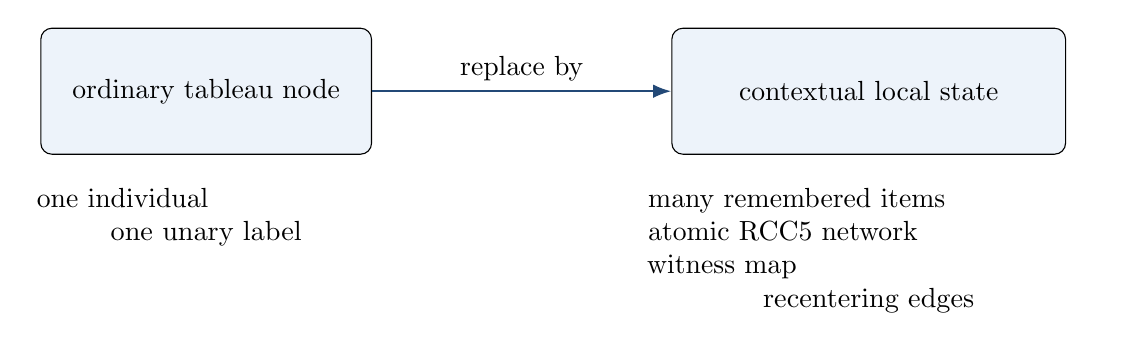
\begin{tikzpicture}[>=Latex, node distance=22mm]
\node[draw, rounded corners, fill=lightaccent, minimum width=42mm, minimum height=16mm] (a) {ordinary tableau node};
\node[draw, rounded corners, fill=lightaccent, minimum width=50mm, minimum height=16mm, right=38mm of a] (b) {contextual local state};
\draw[->, thick, accent] (a) -- node[above, black] {replace by} (b);
\node[below=3mm of a, align=center, text width=43mm] {one individual\newline one unary label};
\node[below=3mm of b, align=center, text width=56mm] {many remembered items\newline atomic RCC5 network\newline witness map\newline recentering edges};
\end{tikzpicture}
\end{center}

An ordinary completion-graph tableau would have to attach a new RCC5 edge from every fresh node to every already existing node. Blocking on unary labels then throws away exactly the information that matters most: how different realizations of the same type sit inside the complete graph. The present calculus caches not raw individuals, but finite remembered contexts.

\section{Open tableau graphs and closed families are the same object}

\begin{definition}[closed family of width $N$]
A \emph{closed family of width $N$} for $C$ is exactly the same data as an open $N$-tableau graph, but viewed non-operationally: a finite set of local states of width at most $N$, a distinguished root state, successor pointers for all items, and recentering maps satisfying \textup{(R1)--(R4)}.
\end{definition}

\begin{proposition}\label{prop:eqv}
For each $N\geq 1$, the following are equivalent:
\begin{enumerate}[label=(\roman*)]
    \item there exists an open $N$-tableau graph for $C$;
    \item there exists a closed family of width $N$ for $C$.
\end{enumerate}
\end{proposition}

\begin{proof}
This is just a change of viewpoint. A finished tableau branch is precisely a rooted finite graph of saturated local states equipped with successor edges and recentering maps. Conversely, any such graph can be read as the result of a tableau run in which all local and global rule obligations have been discharged.
\end{proof}

So soundness of the tableau is exactly the unfolding theorem for closed families.

\section{Unfolding an open tableau graph into a model}

Fix an open $N$-tableau graph $\mathcal T$ with root state $M_\ast$.

\subsection{Witness-generated occurrences}

Only designated center witnesses create new occurrences.

\begin{definition}[occurrences]
The set $\occ(\mathcal T)$ of \emph{occurrences} is the smallest set satisfying:
\begin{enumerate}[label=(O\arabic*)]
    \item the empty word $\epsilon$ lies in $\occ(\mathcal T)$ and carries the root state $M_\epsilon=M_\ast$;
    \item if $\alpha\in \occ(\mathcal T)$ and $\varepsilon=\exists R.D\in \tp_{M_\alpha}(0_{M_\alpha})$, then $\alpha\varepsilon\in \occ(\mathcal T)$ and carries the state
    \[
    M_{\alpha\varepsilon}=\Succ\bigl(M_\alpha,w_{M_\alpha}(\varepsilon)\bigr).
    \]
\end{enumerate}
\end{definition}

Thus $\occ(\mathcal T)$ is the infinite tree of witness-choices through the finite cached tableau graph.

\subsection{Representing descendants in ancestors}

\begin{definition}[representation map]
If $\alpha$ is an ancestor of $\beta$ in $\occ(\mathcal T)$, define an item
\[
\repr_\alpha(\beta)\in I_{M_\alpha}
\]
recursively by:
\begin{enumerate}[label=(P\arabic*)]
    \item $\repr_\alpha(\alpha)=0_{M_\alpha}$;
    \item if $\beta=\alpha\varepsilon\gamma$, then
    \[
    \repr_\alpha(\beta)=u_{M_\alpha,w_{M_\alpha}(\varepsilon)}\bigl(\repr_{\alpha\varepsilon}(\beta)\bigr).
    \]
\end{enumerate}
\end{definition}

\begin{lemma}[representation preserves types and successor states]\label{lem:repr-pres}
If $\alpha$ is an ancestor of $\beta$ and $i=\repr_\alpha(\beta)$, then
\[
\tp_{M_\alpha}(i)=\tp_{M_\beta}(0_{M_\beta})
\qquad\text{and}\qquad
\Succ(M_\alpha,i)=M_\beta.
\]
\end{lemma}

\begin{proof}
By induction on the length of the path from $\alpha$ to $\beta$. The base case is trivial. The induction step uses type preservation and successor preservation in the recentering axioms.
\end{proof}

\begin{lemma}[representation preserves RCC5 labels]\label{lem:repr-rel}
Whenever $\alpha$ is an ancestor of both $\beta$ and $\gamma$,
\[
\rho_{M_\alpha}\bigl(\repr_\alpha(\beta),\repr_\alpha(\gamma)\bigr)
\]
is independent of which chain of recentering maps is used to compute the two representatives.
\end{lemma}

\begin{proof}
Repeated applications of relation preservation show that moving one step upward through a recentering map does not change the RCC5 label between remembered descendants. The statement follows by induction along the unique witness paths.
\end{proof}

\subsection{The induced relation on occurrences}

For arbitrary occurrences $\alpha,\beta\in \occ(\mathcal T)$, let $\delta=\lca(\alpha,\beta)$ be their lowest common ancestor. Define
\[
\mathsf r(\alpha,\beta)=
\rho_{M_\delta}\bigl(\repr_\delta(\alpha),\repr_\delta(\beta)\bigr).
\]
By Lemma~\ref{lem:repr-rel}, this does not depend on any arbitrary choices.

\begin{definition}[occurrence congruence]
Write $\alpha\sim\beta$ iff $\mathsf r(\alpha,\beta)=\Eq$.
\end{definition}

\begin{lemma}[congruence]\label{lem:cong}
$\sim$ is an equivalence relation on $\occ(\mathcal T)$. Moreover, if $\alpha\sim\alpha'$ and $\beta\sim\beta'$, then
\[
\mathsf r(\alpha,\beta)=\mathsf r(\alpha',\beta').
\]
\end{lemma}

\begin{proof}
Reflexivity and symmetry are immediate. For transitivity and congruence, choose one ancestor state that remembers the relevant occurrences and use path consistency of its atomic RCC5 network together with the $\Eq$ row and column of RCC5.
\end{proof}

\subsection{The unfolded interpretation}

\begin{definition}[unfolded model]
The domain of the unfolded interpretation is
\[
\Delta_{\mathcal T}=\occ(\mathcal T)/{\sim}.
\]
For a concept name $A$, define
\[
A^{\mathcal I_{\mathcal T}}
=
\{[\alpha]: A\in \tp_{M_\alpha}(0_{M_\alpha})\}.
\]
For each base relation $R\in \Roles$, define
\[
R^{\mathcal I_{\mathcal T}}
=
\{([\alpha],[\beta]): \mathsf r(\alpha,\beta)=R\}.
\]
By Lemma~\ref{lem:cong}, these definitions are well posed.
\end{definition}

\begin{theorem}[frame soundness]\label{thm:frame}
$\mathcal I_{\mathcal T}$ is a well-defined strong-$\Eq$ $\ALCIRCC$ interpretation.
\end{theorem}

\begin{proof}
The one-cluster condition holds because $\mathsf r(\alpha,\beta)$ is defined for every pair of occurrences. JEPD and converse hold because every local state carries an atomic RCC5 network.

Strong $\Eq$ follows from the quotient construction:
\[
\Eq^{\mathcal I_{\mathcal T}}=
\{([\alpha],[\beta]):\alpha\sim\beta\}
=
\{([\alpha],[\alpha]):[\alpha]\in \Delta_{\mathcal T}\}.
\]

For composition, take
\[
([\alpha],[\beta])\in R^{\mathcal I_{\mathcal T}},
\qquad
([\beta],[\gamma])\in S^{\mathcal I_{\mathcal T}}.
\]
Choose one ancestor occurrence $\delta$ of all three. Then $\delta$ remembers $\alpha,\beta,\gamma$ as items of the path-consistent atomic network $\rho_{M_\delta}$. Hence the third label between $\alpha$ and $\gamma$ belongs to the RCC5 composition entry for $R\circ S$. So the RCC5 table holds in $\mathcal I_{\mathcal T}$.
\end{proof}

\subsection{Truth lemma}

\begin{theorem}[truth lemma]\label{thm:truth}
For every occurrence $\alpha\in \occ(\mathcal T)$ and every formula $D\in \cl(C)$,
\[
D\in \tp_{M_\alpha}(0_{M_\alpha})
\quad\Longrightarrow\quad
[\alpha]\in D^{\mathcal I_{\mathcal T}}.
\]
In particular, if $C\in \tp_{M_\ast}(0_{M_\ast})$, then $\mathcal I_{\mathcal T}\models C$.
\end{theorem}

\begin{proof}
By induction on the structure of $D$.

\emph{Atomic concepts and boolean connectives.} Immediate from the definition of the interpretation of concept names and from the fact that every local item type is Hintikka-saturated.

\emph{Existential restriction.} Suppose $D=\exists R.E$ and $\exists R.E\in \tp_{M_\alpha}(0_{M_\alpha})$. Let $u=w_{M_\alpha}(\exists R.E)$ be the designated witness item. The child occurrence $\beta=\alpha(\exists R.E)$ is centered at the successor state $\Succ(M_\alpha,u)$. By construction,
\[
\mathsf r(\alpha,\beta)=\rho_{M_\alpha}(0_{M_\alpha},u)=R.
\]
Also $E\in \tp_{M_\alpha}(u)=\tp_{M_\beta}(0_{M_\beta})$ by Lemma~\ref{lem:repr-pres}. The induction hypothesis gives $[\beta]\in E^{\mathcal I_{\mathcal T}}$, hence $[\alpha]\in (\exists R.E)^{\mathcal I_{\mathcal T}}$.

\emph{Universal restriction.} Suppose $D=\forall R.E$, $\forall R.E\in \tp_{M_\alpha}(0_{M_\alpha})$, and $([\alpha],[\beta])\in R^{\mathcal I_{\mathcal T}}$. Let $\delta=\lca(\alpha,\beta)$ and set
\[
 i=\repr_\delta(\alpha),
 \qquad
 j=\repr_\delta(\beta).
\]
Then
\[
\tp_{M_\delta}(i)=\tp_{M_\alpha}(0_{M_\alpha}),
\qquad
\rho_{M_\delta}(i,j)=R
\]
by Lemma~\ref{lem:repr-pres} and the definition of $\mathsf r$. Since local states satisfy universal propagation, $E\in \tp_{M_\delta}(j)=\tp_{M_\beta}(0_{M_\beta})$. The induction hypothesis yields $[\beta]\in E^{\mathcal I_{\mathcal T}}$. Therefore $[\alpha]\in (\forall R.E)^{\mathcal I_{\mathcal T}}$.
\end{proof}

Combining Theorems~\ref{thm:frame} and \ref{thm:truth} gives the central soundness statement.

\begin{corollary}[soundness of the tableau]\label{cor:sound}
If there exists an open $N$-tableau graph for $C$, then $C$ is satisfiable in $\ALCIRCC$ under strong $\Eq$ semantics.
\end{corollary}

\section{Conditional completeness and the remaining proof obligation}

Soundness is unconditional. Completeness depends on the width-extraction problem.

\begin{definition}[finite-width extraction statement]
For an input concept $C$, let $\mathsf{FW}(C,N)$ denote the statement:
\begin{quote}
Every model of $C$ contains, after quotienting by a finite descriptor equivalence, a closed family of local states of width at most $N$.
\end{quote}
\end{definition}

This is exactly the point left open in the previous draft, there formulated as a finite quotient lemma.

\begin{proposition}[conditional completeness]\label{prop:condcomplete}
If $\mathsf{FW}(C,N)$ holds, then $C$ is satisfiable if and only if there exists an open $N$-tableau graph for $C$.
\end{proposition}

\begin{proof}
The ``if'' direction is Corollary~\ref{cor:sound}. For the ``only if'' direction, apply $\mathsf{FW}(C,N)$ to obtain a closed family of width at most $N$, then use Proposition~\ref{prop:eqv}.
\end{proof}

\begin{remark}
So the present paper isolates the exact missing ingredient. The tableau calculus itself is not the hard part any more. The hard part is the finite-width extraction theorem from arbitrary models.
\end{remark}

\section{Termination for fixed width}

\begin{proposition}[finite search space for fixed $N$]\label{prop:finite}
For fixed input concept $C$ and fixed width bound $N$, only finitely many pairwise non-isomorphic local states of width at most $N$ exist. Consequently only finitely many rooted finite $N$-tableau graphs exist up to isomorphism.
\end{proposition}

\begin{proof}
There are only finitely many Hintikka types over $\cl(C)$. For a state of width at most $N$, the item set has at most $N$ positions; each position receives one of finitely many types; each ordered pair receives one of finitely many RCC5 labels; and each center existential formula chooses one of at most $N$ witness positions. So only finitely many local-state shapes exist.

For each local-state shape, the number of possible successor edges and recentering maps is finite because the target node must also come from the same finite list and the set of total maps between finite item sets is finite. Hence only finitely many tableau graphs occur up to graph isomorphism.
\end{proof}

\begin{corollary}[conditional decision procedure]
Assume there is a computable bound $N(C)$ such that $\mathsf{FW}(C,N(C))$ holds for every input concept $C$. Then satisfiability in $\ALCIRCC$ is decidable by exhaustive search for an open $N(C)$-tableau graph.
\end{corollary}

\begin{proof}
Proposition~\ref{prop:finite} gives termination of the search at the fixed width $N(C)$, and Proposition~\ref{prop:condcomplete} gives correctness.
\end{proof}

\section{What this note achieves}

The point of the note is not to claim that the final width bound is already known. The point is that the tableau layer is now explicit and cleanly separated from the extraction problem.

What is fully formalized here:
\begin{itemize}
    \item the shape of the local contextual state;
    \item the local saturation rules;
    \item the global successor / recentering / caching rules;
    \item the exact object recognized by the tableau (an open $N$-tableau graph);
    \item the full unfolding soundness theorem from open tableaux to genuine models.
\end{itemize}

What still needs to be proved to obtain a finished decidability theorem:
\begin{itemize}
    \item a model-extraction theorem showing that every satisfiable concept admits a finite-width closed family, together with a computable bound $N(C)$.
\end{itemize}

That is the single remaining global proof obligation.

\begin{thebibliography}{9}

\bibitem{Wessel2003}
Michael Wessel.
\newblock \emph{Qualitative Spatial Reasoning with the ALCIRCC Family -- First Results and Unanswered Questions}.
\newblock Technical Report FBI-HH-M-324/03, University of Hamburg, 2002/2003.

\bibitem{Claude2026}
Claude.
\newblock \emph{On the Decidability of ALCIRCC5 and ALCIRCC8: Quasimodels Meet the Patchwork Property}.
\newblock Discussion draft, 2026.

\end{thebibliography}

\end{document}
